\documentclass{beamer}

\usepackage[utf8]{inputenc}
\usepackage{amsmath,amsthm}
\usepackage{amssymb}
\usepackage{bbm}
\usepackage{amsfonts}
\usepackage{wasysym}

\usepackage{xcolor}
\definecolor{lightred}{RGB}{209,105,81}
\definecolor{lightgreen}{RGB}{58,181,75}
\definecolor{thickblue}{RGB}{5,43,108}
\definecolor{fairblue}{RGB}{0,112,192}
\definecolor{lightblue}{RGB}{0,153,228}
\definecolor{light_red}{RGB}{209,105,81}
\definecolor{light_green}{RGB}{58,181,75}
\definecolor{thick_blue}{RGB}{5,43,108}
\definecolor{fair_blue}{RGB}{0,112,192}
\definecolor{light_blue}{RGB}{0,153,228}

\usepackage{graphicx}
\graphicspath{ {./graphics/} }

% \usepackage{enumitem}
\usepackage{pifont}


\setbeamertemplate{frametitle}[default][center]
\setbeamertemplate{navigation symbols}{}
\setbeamerfont{footline}{series=\bfseries}
\setbeamertemplate{footline}[page number]

\usepackage{tikz}
\newcommand{\topline}{%
  \tikz[remember picture, overlay] {%
    \draw[gray, thick] ([xshift=1cm,yshift=-1.2cm]current page.north west)
             -- ([xshift=-1cm,yshift=-1.2cm,xshift=\paperwidth]current page.north west);}}
             
             
%Information to be included in the title page:
\title{\color{lightred}\textbf{An Introduction to Social Learning}}

\author{Xinyu Chen}

\vspace{-10em}
% \institute{Overleaf}
\date{ }



\begin{document}

\begin{frame}

\begin{center}
{\color{black}\LARGE\textbf{Social Learning}}
    
\vspace{0.8em}

{\color{fairblue}\large\textbf{Theory and Its Applications to Transportation}}
    
\vspace{1em}
    
\textbf{\color{gray}Xinyu Chen}

\vspace{0.4em}

\textbf{\color{gray}Polytechnique Montreal}

\end{center}


\centering

% \includegraphics[scale=0.2]{graphics/citibike_travel.png}

\end{frame}


\begin{frame}
\frametitle{\color{lightred}\textbf{Outline}}
\topline

\begin{itemize}
\item {\color{light_red}Background}
\item {\color{light_red}Bobo doll experiments}
\item {\color{light_red}People can learn through observation}
\item {\color{light_red}Sustainable transport innovations}
\item {\color{light_red}An interesting research idea}
\end{itemize}

\end{frame} 


\begin{frame}
\frametitle{\color{lightred}\textbf{Background}}
\topline

\resizebox{11cm}{!}{
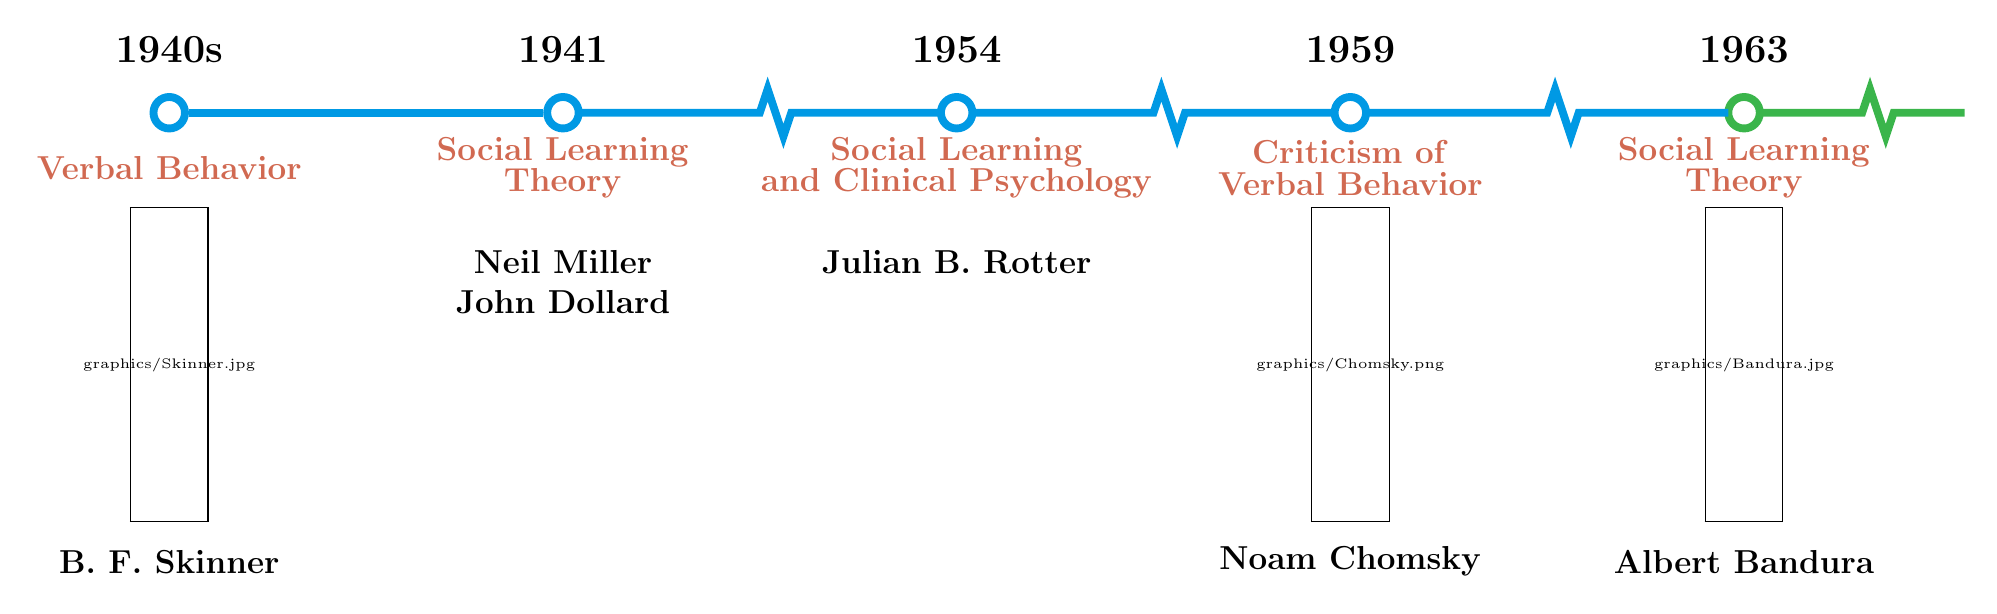
\begin{tikzpicture}

%%% B. F. Skinner %%%
\pgfdeclareimage[height = 4cm]{skinner}{graphics/Skinner.jpg}
\draw (0, 2.5) node {\color{light_red}\textbf{\large{Verbal Behavior}}};
\node (skinner) at (0, 0) {\pgfuseimage{skinner}};
\draw (0, -2.5) node {\large\textbf{B. F. Skinner}};

\node [circle, line width = 1mm, draw = light_blue, fill = white, minimum size = 0.4cm] (node1) at (0, 3.2) {};
\draw (0, 4) node {\Large\textbf{1940s}};

%%% Social Learning book 1 %%%
\node [circle, line width = 1mm, draw = light_blue, fill = white, minimum size = 0.4cm] (node2) at (5, 3.2) {};
\draw (5, 4) node {\Large\textbf{1941}};
\draw (5, 2.7) node {\color{light_red}\textbf{\large{Social Learning}}};
\draw (5, 2.3) node {\color{light_red}\textbf{\large{Theory}}};
\draw (5, 1.3) node {\large\textbf{Neil Miller}};
\draw (5, 0.8) node {\large\textbf{John Dollard}};

%%% Path between Skinner and Social Learning book 1 %%%
\path [line width = 1mm, draw = light_blue, -] (node1) edge (node2);

%%% Social Learning book 2 %%%
\node [circle, line width = 1mm, draw = light_blue, fill = white, minimum size = 0.4cm] (node3) at (10, 3.2) {};
\draw (10, 4) node {\Large\textbf{1954}};
\draw (10, 2.7) node {\color{light_red}\textbf{\large{Social Learning}}};
\draw (10, 2.3) node {\color{light_red}\textbf{\large{and Clinical Psychology}}};
\draw (10, 1.3) node {\large\textbf{Julian B. Rotter}};

%%% Path between book 1 and book 2 %%%
\draw [line width = 1mm, draw = light_blue]  (5.2, 3.2) -- (7.5, 3.2) -- (7.6, 3.5) -- (7.8, 2.9) -- (7.9, 3.2) -- (9.8, 3.2);

%%% Noam Chomsky %%%
\pgfdeclareimage[height = 4cm]{chomsky}{graphics/Chomsky.png}
\node (chomsky) at (15, 0) {\pgfuseimage{chomsky}};
\node [circle, line width = 1mm, draw = light_blue, fill = white, minimum size = 0.4cm] (node4) at (15, 3.2) {};
\draw (15, 4) node {\Large\textbf{1959}};
\draw (15, 2.7) node {\color{light_red}\textbf{\large{Criticism of}}};
\draw (15, 2.3) node {\color{light_red}\textbf{\large{Verbal Behavior}}};
\draw (15, -2.5) node {\large\textbf{Noam Chomsky}};

%%% Path between book 2 and Chomsky %%%
\draw [line width = 1mm, draw = light_blue]  (5.2 + 5, 3.2) -- (7.5 + 5, 3.2) -- (7.6 + 5, 3.5) -- (7.8 + 5, 2.9) -- (7.9 + 5, 3.2) -- (9.8 + 5, 3.2);

%%% Albert Bandura %%%
\pgfdeclareimage[height = 4cm]{bandura}{graphics/Bandura.jpg}
\node (bandura) at (20, 0) {\pgfuseimage{bandura}};
\node [circle, line width = 1mm, draw = light_green, fill = white, minimum size = 0.4cm] (node5) at (20, 3.2) {};
\draw (20, 4) node {\Large\textbf{1963}};
\draw (20, 2.7) node {\color{light_red}\textbf{\large{Social Learning}}};
\draw (20, 2.3) node {\color{light_red}\textbf{\large{Theory}}};
\draw (20, -2.5) node {\large\textbf{Albert Bandura}};

%%% Path between Chomsky and Bandura %%%
\draw [line width = 1mm, draw = light_blue]  (5.2 + 10, 3.2) -- (7.5 + 10, 3.2) -- (7.6 + 10, 3.5) -- (7.8 + 10, 2.9) -- (7.9 + 10, 3.2) -- (9.8 + 10, 3.2);

%%% Path between Chomsky and Bandura %%%
\draw [line width = 1mm, draw = light_green]  (5.2 + 15, 3.2) -- (6.5 + 15, 3.2) -- (6.6 + 15, 3.5) -- (6.8 + 15, 2.9) -- (6.9 + 15, 3.2) -- (7.8 + 15, 3.2);

\end{tikzpicture}
}

\noindent\rule[0ex]{\linewidth}{0.2pt}

\vspace{0.8em}

\small

{\color{black}Contribution of Bandura's Theory:}

\vspace{0.5em}

\centering

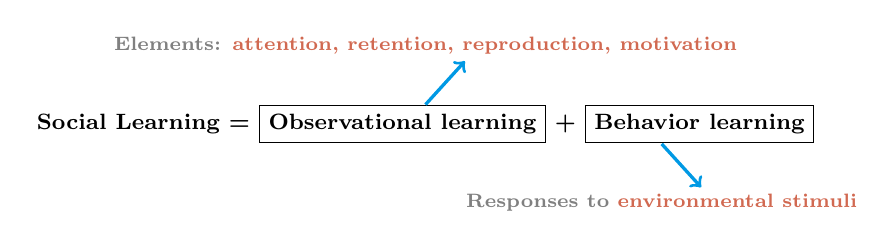
\begin{tikzpicture}
\draw (0, 0) node {\footnotesize\textbf{Social Learning = \fbox{Observational learning} + \fbox{Behavior learning}}};
\draw (0, 1) node {\scriptsize{\textbf{\color{gray}Elements: \color{light_red}attention, retention, reproduction, motivation}}};
\draw [very thick, draw = light_blue, ->]  (0, 0.25) -- (0.5, 0.8);

\draw (3, -1) node {\scriptsize{\textbf{\color{gray}Responses to \color{light_red}environmental stimuli}}};
\draw [very thick, draw = light_blue, ->]  (3, -0.25) -- (3.5, -0.8);

\end{tikzpicture}

\end{frame}


\begin{frame}
\frametitle{\color{light_red}\textbf{Bobo Doll Experiments}}
\topline

\begin{columns}
\begin{column}{0.3\textwidth}
\centering
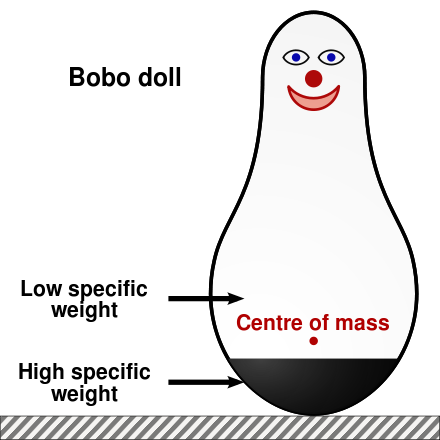
\includegraphics[scale = 0.2]{graphics/bobo_doll.png}

\end{column}
\begin{column}{0.7\textwidth}
\centering
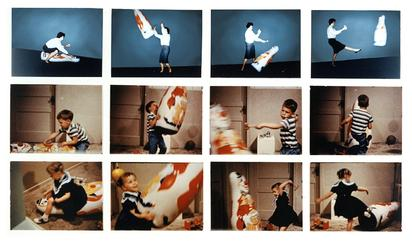
\includegraphics[scale = 0.45]{graphics/bobo_doll_experiment.jpg}
\end{column}
\end{columns}

\noindent\rule[0ex]{\linewidth}{0.2pt}

\vspace{0.8em}

\small

\pause

{\color{black}Contribution of Bandura's Theory:}

\vspace{0.5em}

\centering

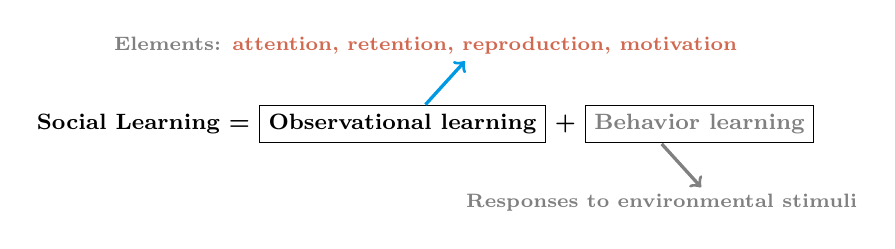
\begin{tikzpicture}
\draw (0, 0) node {\footnotesize\textbf{Social Learning = \fbox{Observational learning} + \fbox{\color{gray}Behavior learning}}};
\draw (0, 1) node {\scriptsize{\textbf{\color{gray}Elements: \color{light_red}attention, retention, reproduction, motivation}}};
\draw [very thick, draw = light_blue, ->]  (0, 0.25) -- (0.5, 0.8);

\draw (3, -1) node {\scriptsize{\textbf{\color{gray}Responses to environmental stimuli}}};
\draw [very thick, draw = gray, ->]  (3, -0.25) -- (3.5, -0.8);

\end{tikzpicture}

\end{frame}


\begin{frame}
\frametitle{\color{light_red}\textbf{People Can Learn Through Observation}}
\topline

% \centering
\begin{center}
\includegraphics[width = 0.85\textwidth]{graphics/use_chopsticks.png}
\end{center}

\vspace{0.5em}

\pause

\footnotesize
\textbf{\color{gray}Elements of social learning:}
\scriptsize
\begin{itemize}
    \item[\ding{212}] \textbf{\color{light_red}Attention:} {\color{light_blue}\scriptsize{Dedicate attention to learning.}}
    \item[\ding{212}] \textbf{\color{light_red}Retention:} {\color{light_blue}\scriptsize{Ability to store information.}}
    \item[\ding{212}] \textbf{\color{light_red}Reproduction:} {\color{light_blue}\scriptsize{Perform the behavior you observed.}}
    \item[\ding{212}] \textbf{\color{light_red}Motivation:} {\color{light_blue}\scriptsize{Be motivated to imitate the behavior that has been modeled.}}
\end{itemize}

\end{frame}


\begin{frame}

\frametitle{\color{light_red}\textbf{- Sustainable Transport Innovations}}
\topline

{\footnotesize\color{thick_blue}\textbf{- Sustainable transport projects} (Netherlands)\footnote{\scriptsize{\color{black!75}J.C.J.M. van den Bergh et al., Social learning by doing in sustainable transport innovations: Ex-post analysis of common factors behind successes and failures. Research Policy, 2007, 36: 247-259.}}:}

\vspace{0.5em}

\resizebox{10.5cm}{!}{
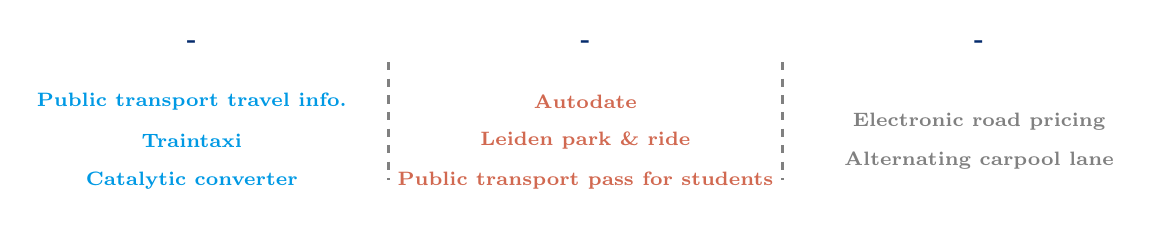
\begin{tikzpicture}
\draw (0, 0.75) node {\small\textbf{\color{thick_blue}-}};
\draw (0, 0) node {\scriptsize\textbf{\color{light_blue}Public transport travel info.}};
\draw (0, -0.5) node {\scriptsize\textbf{\color{light_blue}Traintaxi}};
\draw (0, -1.0) node {\scriptsize\textbf{\color{light_blue}Catalytic converter}};
\draw [very thick, draw = gray, dashed]  (2.5, 0.5) -- (2.5, -1.0);

\draw (5, 0.75) node {\small\textbf{\color{thick_blue}-}};
\draw (5, 0) node {\scriptsize\textbf{\color{light_red}Autodate}};
\draw (5, -0.5) node {\scriptsize\textbf{\color{light_red}Leiden park \& ride}};
\draw (5, -1.0) node {\scriptsize\textbf{\color{light_red}Public transport pass for students}};
\draw [very thick, draw = gray, dashed]  (7.5, 0.5) -- (7.5, -1.0);

\draw (10, 0.75) node {\small\textbf{\color{thick_blue}-}};
\draw (10, -0.25) node {\scriptsize\textbf{\color{gray}Electronic road pricing}};
\draw (10, -0.75) node {\scriptsize\textbf{\color{gray}Alternating carpool lane}};

\end{tikzpicture}
}

\vspace{-0.2em}

\noindent\rule[0ex]{\linewidth}{0.2pt}

\vspace{0.5em}

{\footnotesize\color{thick_blue}\textbf{- How to do?}}

\begin{itemize}\footnotesize
    \item[\ding{212}] {\color{fair_blue}Identify sustainable transport innovation projects}
    \item[\ding{212}] {\color{fair_blue}Define factors} {\scriptsize\color{gray}(e.g., technological, administrative, political, economic)}
    \item[\ding{212}] {\color{fair_blue}Collect data from interviewees}
    \item[\ding{212}] {\color{fair_blue}Apply social learning mechanism}
\end{itemize}

\end{frame}


\begin{frame}

\frametitle{\color{light_red}\textbf{- Sustainable Transport Innovations}}
\topline

{\footnotesize\color{thick_blue}\textbf{- Sustainable transport projects} (Netherlands)\footnote{\scriptsize{\color{black!75}J.C.J.M. van den Bergh et al., Social learning by doing in sustainable transport innovations: Ex-post analysis of common factors behind successes and failures. Research Policy, 2007, 36: 247-259.}}:}

\vspace{0.5em}

\resizebox{11cm}{!}{
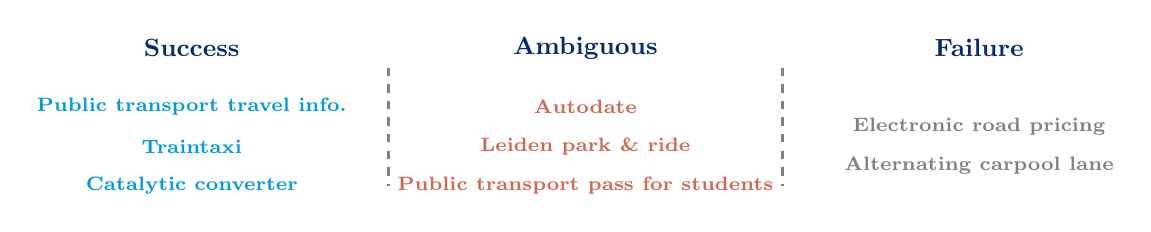
\begin{tikzpicture}
\draw (0, 0.75) node {\small\textbf{\color{thick_blue}Success}};
\draw (0, 0) node {\scriptsize\textbf{\color{light_blue}Public transport travel info.}};
\draw (0, -0.5) node {\scriptsize\textbf{\color{light_blue}Traintaxi}};
\draw (0, -1.0) node {\scriptsize\textbf{\color{light_blue}Catalytic converter}};
\draw [very thick, draw = gray, dashed]  (2.5, 0.5) -- (2.5, -1.0);

\draw (5, 0.75) node {\small\textbf{\color{thick_blue}Ambiguous}};
\draw (5, 0) node {\scriptsize\textbf{\color{light_red}Autodate}};
\draw (5, -0.5) node {\scriptsize\textbf{\color{light_red}Leiden park \& ride}};
\draw (5, -1.0) node {\scriptsize\textbf{\color{light_red}Public transport pass for students}};
\draw [very thick, draw = gray, dashed]  (7.5, 0.5) -- (7.5, -1.0);

\draw (10, 0.75) node {\small\textbf{\color{thick_blue}Failure}};
\draw (10, -0.25) node {\scriptsize\textbf{\color{gray}Electronic road pricing}};
\draw (10, -0.75) node {\scriptsize\textbf{\color{gray}Alternating carpool lane}};

\end{tikzpicture}
}

\vspace{-0.2em}

\noindent\rule[0ex]{\linewidth}{0.2pt}

\vspace{0.5em}

{\footnotesize\color{thick_blue}\textbf{- Findings by using social learning:}}

\begin{itemize}\footnotesize
    \item[\ding{212}] {\color{fair_blue}Predominant factors:{\color{gray}\scriptsize Political, process-related, socio-cultural, and psychological factors}}
    \item[\ding{212}]{\color{fair_blue}Less important factors:{\color{gray}\scriptsize Technical and economic factors}}
    \item[\ding{212}] {\color{fair_blue}Communication is an important element of social learning to foster innovations.}
\end{itemize}

\end{frame}


% \begin{frame}

% \frametitle{\color{light_red}\textbf{Modeling Travellers' Change of Behaviour}}
% \topline

% Incorporating social interaction and social learning in modeling ...

% Social interaction is a medium for social learning to happen.

% - 1st level: an interdependent situation where travellers are in a similar transport system with other travellers.

% - 2nd level: happen through observation by a traveller of other travellers' choices without involving processes of communications.

% Social learning: Individuals learn from others' experiences or observed behaviours.

% Uncertainty:

% - Effects of natural events (e.g., rain, snow)

% - Effects of human-made events (e.g., accidents, roadworks)

% - Travellers' choices

% Uncertainties contribute to the complex and dynamic process of travel behavioural change

% \end{frame}


% \begin{frame}
% \frametitle{\color{light_red}\textbf{Modeling Travellers' Change of Behavior}}
% \topline

% \textbf{\color{light_green}Laboratory experiment:}

% \begin{itemize}\footnotesize
%     \item[\ding{212}] Computer interface based on Z-tree
%     \item[\ding{212}] Simulates a repeated decision-making environments.
%     \item[\ding{212}] Whether or not contribute to an employer-based demand management initiative to reduce employees' car-use.
%     \item[\ding{212}] Two schemes of social information about other participants' behaviour.
% \end{itemize}

% \textbf{\color{light_green}Simulation experiment:}

% \begin{itemize}\footnotesize
% \item[\ding{212}] A larger system with more individuals
% \item[\ding{212}] Individual layer + interaction layer
% \end{itemize}


% \end{frame}


\begin{frame}
\frametitle{\textbf{\color{light_red}A Potential Research Idea}}
\topline

\begin{columns}
\begin{column}{0.3\textwidth}
\centering

\includegraphics[scale = 0.2]{graphics/wechat.png}
\end{column}
\begin{column}{0.6\textwidth}
\centering
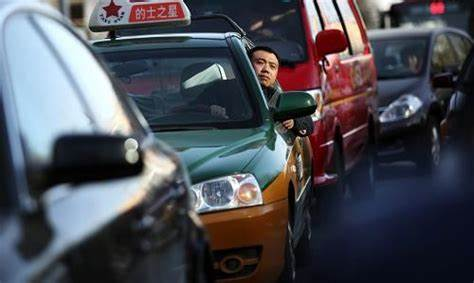
\includegraphics[scale = 0.28]{graphics/congested_taxi.jpeg}
\end{column}
\end{columns}

\vspace{0.5em}

\noindent\rule[0ex]{\linewidth}{0.2pt}

\vspace{0.2em}

\begin{block}{\color{black}\footnotesize[Idea] {\color{light_red}\textbf{Social learning and social network of taxi drivers}}\footnote{\scriptsize{\color{black!75}Y. Sunitiyoso, et al., On the potential for recognising of social interaction and social learning in modelling travellers’ change of behaviour under uncertainty. Transportmetrica, 2011, 7(1): 5-30.}}}
\vspace{0.5em}
\color{light_blue}
\beamergotobutton{Idea from} \footnotesize In China, it is very common that taxi drivers have some certain Wechat teams for \textbf{communication}. They share and discuss \textbf{travel demands} and \textbf{traffic conditions} with other taxi drivers on Wechat.
\end{block}

\vspace{0.3em}

\footnotesize[Question] {\color{light_red}Can social learning and social network help \textbf{improve the income of taxi drivers}?}

\end{frame}


\begin{frame}
\frametitle{\color{lightred}\textbf{Reference}}
\topline

\footnotesize
\begin{enumerate}
    \item Social learning on wikipedia. [\href{https://en.wikipedia.org/wiki/Social_learning_theory}{\color{blue!80!black}website}]
    \item Bobo doll experiment on wikipedia. [\href{https://en.wikipedia.org/wiki/Bobo_doll_experiment}{\color{blue!80!black}website}]
    \item How social learning theory works. [\href{https://www.verywellmind.com/social-learning-theory-2795074}{\color{blue!80!black}post}]
    \item How observational learning affects behavior. [\href{https://www.verywellmind.com/what-is-observational-learning-2795402}{\color{blue!80!black}post}]
    \item J.C.J.M. van den Bergh et al., Social learning by doing in sustainable transport innovations: Ex-post analysis of common factors behind successes and failures. Research Policy, 2007, 36: 247-259.
    \item Y. Sunitiyoso, et al., On the potential for recognising of social interaction and social learning in modelling travellers’ change of behaviour under uncertainty. Transportmetrica, 2011, 7(1): 5-30.
\end{enumerate}

\end{frame}


\begin{frame}

\vspace{2em}

\centering\Large {\textbf{\color{lightred}Thanks for your attention!}}

% \vspace{0.5em}

% \footnotesize
% {\color{gray}LaTeX codes for creating these slides are publicly available at:}

\end{frame}



\end{document}